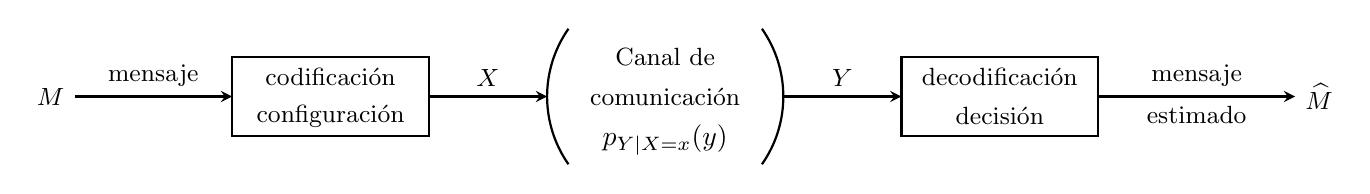
\begin{tikzpicture}
\shorthandoff{>}
%
% Mensaje
\draw[>=stealth,->,thick] (0,0) node[left]{\small $M$} --(2,0);
\node[above] at (1,0){\small mensaje};
%
% codificacion
\draw[thick] (2,-.5) rectangle (4.5,.5);
\node at (3.25,.25){\small codificaci\'on};
\node at (3.25,-.25){\small configuraci\'on};
%
% entrada del canal
\draw[>=stealth,->,thick] (4.5,0)--(6,0);
\node[above] at (5.25,0){\small $X$};
%
% Canal de com
\pgfmathsetmacro{\t}{35};
\pgfmathsetmacro{\r}{1.5};
\draw[thick] ({6+\r*(1+cos(180-\t))},{\r*sin(\t)}) arc (180-\t:180+\t:\r);
\draw[thick] ({6+\r*(1+cos(\t))},{-\r*sin(\t)}) arc (-\t:\t:\r);
\node at ({6+\r},.5){\small Canal de};
\node at ({6+\r},0){\small comunicaci\'on};
\node at ({6+\r},-.55){$p_{Y|X=x}(y)$};
%
% salida
\draw[>=stealth,->,thick] ({6+2*\r},0)--({7.5+2*\r},0);
\node[above] at ({6.75+2*\r},0){\small $Y$};
%
% decodificacion/decision
\draw[thick] ({7.5+2*\r},-.5) rectangle ({10+2*\r},.5);
\node at ({8.75+2*\r},.25){\small decodificaci\'on};
\node at ({8.75+2*\r},-.25){\small decisi\'on};
%
% Mensaje estimado
\draw[>=stealth,->,thick] ({10+2*\r},0)--({12.5+2*\r},0) node[right]{\small $\widehat{M}$};
\node[above] at ({11.25+2*\r},0){\small mensaje};
\node[below] at ({11.25+2*\r},0){\small estimado};
\end{tikzpicture}
